%%%%%%%%%%%%%%%%%%%%%%%%%%%%% Define Article %%%%%%%%%%%%%%%%%%%%%%%%%%%%%%%%%%
\documentclass{article}
%%%%%%%%%%%%%%%%%%%%%%%%%%%%%%%%%%%%%%%%%%%%%%%%%%%%%%%%%%%%%%%%%%%%%%%%%%%%%%%

%%%%%%%%%%%%%%%%%%%%%%%%%%%%% Using Packages %%%%%%%%%%%%%%%%%%%%%%%%%%%%%%%%%%
\usepackage{listings, xcolor}
\usepackage{parskip}
\usepackage{hyperref}
\usepackage{amsmath}
\usepackage{graphicx}
\usepackage[a4paper, margin = 1.5cm]{geometry}
\usepackage{float}
\usepackage{amssymb}

%%%%%%%%%%%%%%%%%%%%%%%%%%%%%%% Title & Author %%%%%%%%%%%%%%%%%%%%%%%%%%%%%%%%
\title{Tipologie di Requisiti}
\author{Trentin Tommaso}
%%%%%%%%%%%%%%%%%%%%%%%%%%%%%%%%%%%%%%%%%%%%%%%%%%%%%%%%%%%%%%%%%%%%%%%%%%%%%%%

\begin{document}
  \maketitle
  \tableofcontents
  \newpage
  \section{Definizione di Requisiti}
    Requisiti non sono solo le funzionalità. Vanno definite esigenze del cliente che il sistema deve fornire ed entro quali vincoli operativi (se sistema funziona correttamente ma non rispetta vincoli, non sarà di interesse per il cliente). \\
    Vincolo: \textbf{Descrizione di qualcosa che sistema dovrà fare / di una proprietà o vincolo operativo che si desidera}, può indicare diverse tipologie di descrizione:
    \begin{itemize}
      \item Formulazione astratta e ad alto livello, spesso in linguaggio naturale;
      \item Specifica dettagliata, in linguaggio formale matematico.
    \end{itemize}
    Definizione ampia necessaria poiché un requisito può avere vari scopi nella patica:
    \begin{itemize}
      \item Base per una gara fra fornitori concorrenti, quindi aperto a interpretazioni diverse;
      \item Base del contratto stesso (dopo assegnazione appalto), pertanto da definire in dettaglio.
    \end{itemize}
    \textbf{Ingegneria dei requisiti} è processo di ricerca, analisi, documentazione e verifica requisiti, tale processo finalizzato a stabilire funzionalità dl SW, vincoli operativi e vincoli per lo sviluppo. 
    \subsection{Requisiti Utente}
      \begin{itemize}
        \item Frasi in linguaggio naturale (correlate da diagrammi) relative a funzionalità che sistema deve fornire e suoi vincoli operativi;
        \item Generalmente ad alto livello (possono contenere dettagli);
        \item Descritti solamente mediante linguaggio naturale e diagrammi \textit{comprensibili a tutti gli utenti}, anche a quelli privi di dettagliate conoscenze tecniche.
      \end{itemize}
    \subsection{Requisiti di Sistema}
      \begin{itemize}
        \item Documento strutturato che fornisce descrizione dettagliata di funzionalità sistema / vincoli operativi;
        \item Definisce cosa andrà sviluppato;
        \item Può essere parte del contratto utente-sviluppatore. 
      \end{itemize}
  \section{Requisiti Funzionali / Non Funzionali}
    \subsection{Requisiti Funzionali}
      Descrivono funzionalità che dovranno essere offerte dal sistema, possono essere espressi a due livelli di astrazione:
      \begin{itemize}
        \item \textbf{Requisiti funzionali all'utente}: descrizioni di alto livello su ciò che il sistema fa;
        \item \textbf{Requisiti funzionali di sistema}: descrizioni dettagliate delle funzionalità (comprensive di input, output, eccezioni). 
      \end{itemize}
    \subsection{Completezza / Consistenza dei Requisiti}
      Requisiti imprecisi o ambigui possono essere implementati in modi diversi da diversi stakeholders, pertanto specifiche dei requisiti devono essre:
      \begin{itemize}
        \item \textbf{Complete}: tutti requisiti richiesti dai clienti devono essere presenti;
        \item \textbf{Consistenti}: requisiti non devono avere definizioni contraddittorie o essere in conflitto. 
      \end{itemize}
      Nella realtà è facile commettere errori / omissioni, soprattutto per sistemi complessi e di grandi dimensioni, alcune incoerenze possono invece emergere soltanto durante lo sviluppo del sistema (specialmente con stakeholder con aspettative differenti / contrastanti). 
    \subsection{Requisiti Non Funzionali}
      Non riguardano direttamente funzionalità offerte dal sistema ma definiscono proprietà / vincoli del sistema e del suo processo di sviluppo:
      \begin{itemize}
        \item Proprietà del sistema: affidabilità, tempi di risposta e uso memoria, \dots;
        \item Vincoli del sistema: capacità dispositivi I/O, rappresentazione dati, \dots;
        \item Vincoli processo di sviluppo: uso particolari standard per documentazione, linguaggi di programmazione specifici, \dots
      \end{itemize}
      Possono essere più critici dei requisiti funzionali dato che, se non soddisfatti, il sistema potrebbe risultare inutilizzabile. 
      \subsubsection{Tipi di Requisiti Non Funzionali}
        \begin{itemize}
          \item \textbf{Requisiti del prodotto}: derivano da caratteristiche SW richieste, specificano comportamento del prodotto;
          \item \textbf{Requisiti organizzativi}: derivano da politiche e procedure dell'organizzazione che utilizza SW e del cliente (standard di processi, piattaforme e linguaggi di programmazione);
          \item \textbf{Requisiti esterni}: tutti requisiti che derivano da fattori esterni al sistema e al suo processo di sviluppo (requisiti legislativi da rispettare, requisiti etici che garantiscono accettazione del sistema).
        \end{itemize}
        \begin{figure}[h!]
          \begin{center}
            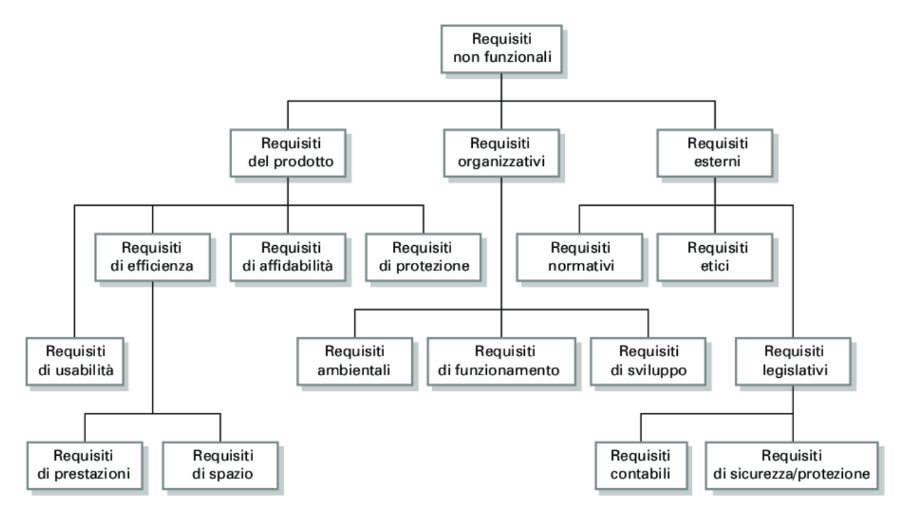
\includegraphics[width=0.5\textwidth]{./figures/req_nf.png}
          \end{center}
        \end{figure}
      \subsubsection{Verificabilità dei Requisiti}
        Requisiti non funzionali possono essere difficili da definire precisamente, quindi difficili da verificare:
        \begin{itemize}
          \item Cliente potrebbe specificarli come \textbf{obiettivi} generici / vaghi, causando problemi agli sviluppatori a causa della libera interpretazione;
          \item Bisognerebbe descrivere requisiti non funzionali quantitativamente, in modo che possano essere \textbf{verficabili} $\rightarrow$ devono contenere una misura in qualche modo verificabile:
            \begin{itemize}
              \item \textit{Velocità} - Transazioni\/s, tempi di risposta, tempo di refresh sullo schermo;
              \item \textit{Dimensione} - MB \/ numero di chip ROM;
              \item \textit{Facilità d'uso} - Tempo di addestramento, numero di maschere d'aiuto;
              \item \textit{Affidabilità} - Tempo medio di funzionamento, portabilità di indisponibilità, tasso di malfunzionamento, disponibilità;
              \item \textit{Robustezza} - Tempo di riavvio dopo malfunzionamento, percentuale di eventi che causano malfunzionamenti, probabilità di corruzione dati dopo un malfunzionamento;
              \item \textit{Portabilità} - Percentuale di istruzioni dipendenti dal sistema target, numero di sistemi target.
            \end{itemize}
        \end{itemize}
      \subsubsection{Requisiti di Dominio}
        Requisiti funzionali / non funzionali e vincoli che derivano dal dominio applicativo del sistema (e non dalle esigenze utente), talvolta ovvie per gli esperti (ma non per gli sviluppatori) e quindi tralasciate. Solitamente espressi nel linguaggio estremamente specializzato del dominio, possono far riferimento a concetti specifici del dominio.
  \section{Ingegneria dei Requisiti}
    Idea- 3 attività chiave:
    \begin{itemize}
      \item \textbf{Deduzione e analisi dei requisiti} - comprensione requisiti mediante interazione con stakeholder;
      \item \textbf{Specifica dei requisiti} - traduzione requisiti in specifiche in un formato coerente;
      \item \textbf{Convalida dei requisiti} - controllo che requisiti corrispondano a richieste cliente.
    \end{itemize}
    \subsection{Modello sequenziale}
      Le tre attività sono \textit{per forza} sequenziali.
      \begin{figure}[htpb]
          \centering
          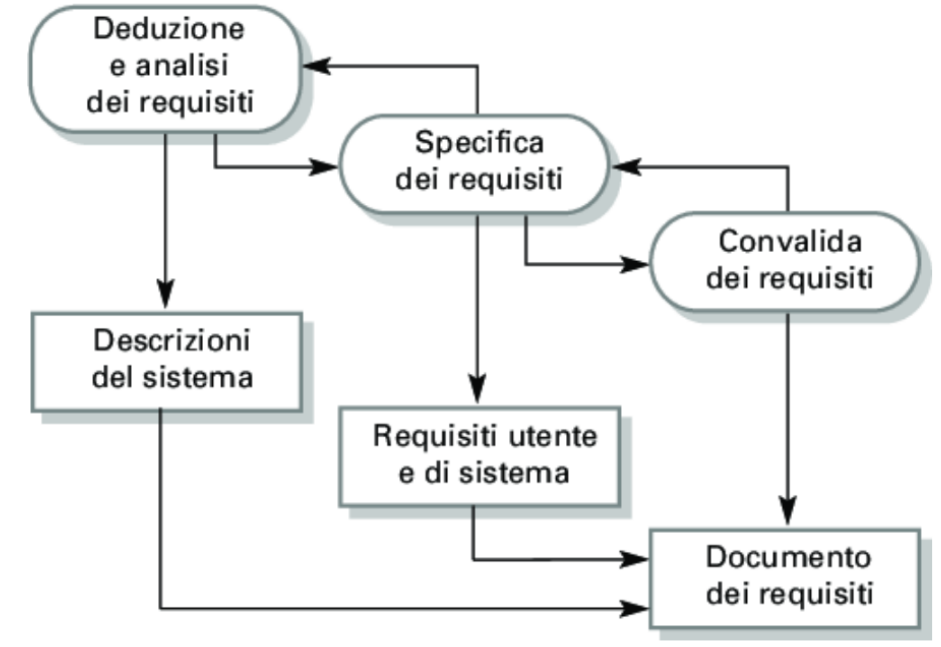
\includegraphics[width=0.5\linewidth]{figures/mod_seq.png}
      \end{figure}
    \subsection{Modello a spirale}
      Processo di ingegneria dei requisiti è nella pratica spesso fortemente iterativo (e con fasi interlacciate), viene quindi utilizzato un modello a spirale quando i requisiti sono sviluppati con diversi livelli di dettaglio (generali, utente, sistema). 
      \begin{figure}[htpb]
          \centering
          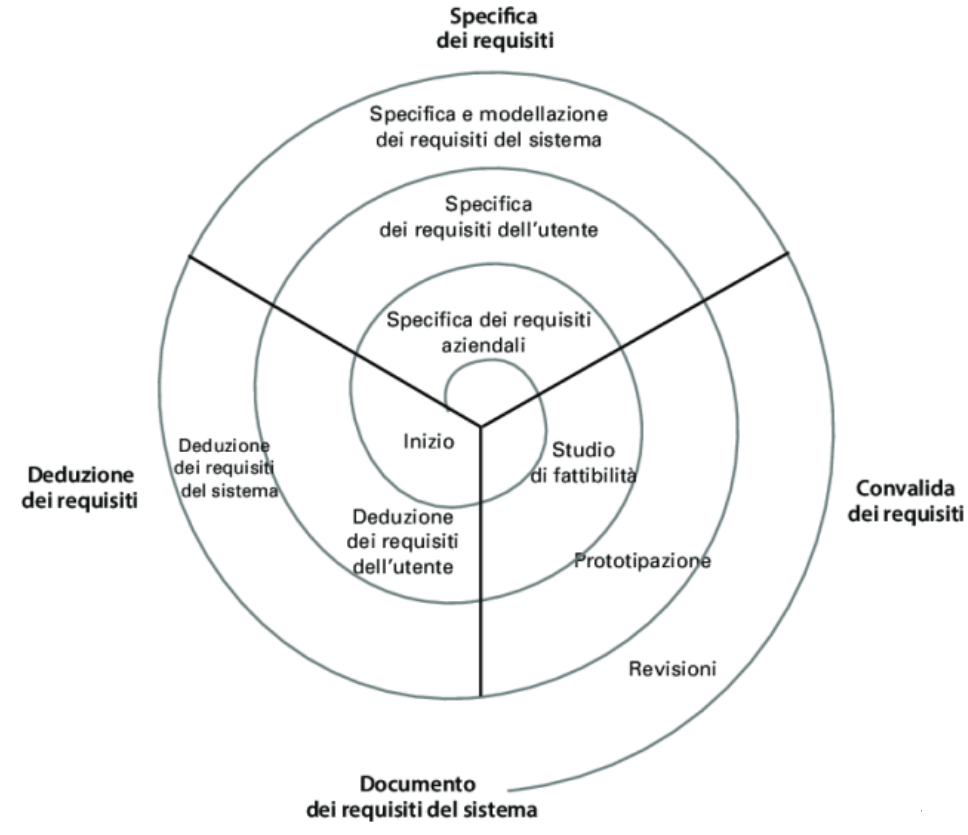
\includegraphics[width=0.5\linewidth]{figures/mod_spir.png}
      \end{figure}
    \subsection{Ingegneria dei requisiti - Metodi agili}
      Nei metodi agili la specifica dei requisiti non è un'attività separata (considerata parte dello sviluppo), i requisiti sono specificati informalmente per ciascun incremento del sistema, in base alle priorità utente.
\end{document}
